\documentclass[tikz, border = 1 cm]{standalone}

%%%%%%%%%%%%%%
\usepackage{tikz}
\usetikzlibrary{calc}
\usetikzlibrary{positioning}
%%%%%%%%%%%%%%

%%%%%%%%%%%%%%
\definecolor{blue1}		{RGB}{0,177,234}
\definecolor{orange1}	{RGB}{255,126,46}
%%%%%%%%%%%%%%

%%%%%%%%%%%%%%
\tikzset{node distance=0.75cm and 2.0cm}

\tikzstyle{branch}= 	[line width=1.75pt]
\tikzstyle{commit}=	[circle, inner sep=0pt, text width=8pt, align=center]
\tikzstyle{hash}=	[font=\scriptsize, yshift=-0.25cm]
\tikzstyle{bname}=	[text width=0.5cm, inner sep=0pt, font=\bfseries\linespread{1.0}\selectfont]

\tikzstyle{cmaster}=	[commit, fill=blue1, draw=blue1]
\tikzstyle{bmaster}=	[branch, draw=blue1]
\tikzstyle{nmaster}=	[bname, text=blue1]

\tikzstyle{ctop}=		[commit, fill=orange1, draw=orange1]
\tikzstyle{btop}=	[branch, draw=orange1]
\tikzstyle{ntop}=	[bname, text=orange1]
%%%%%%%%%%%%%%

%%%%%%%%%%%%%%
%%%%%%%%%%%%%%
%%%%%%%%%%%%%%
\begin{document}

%%%%%%%%%%%%%%
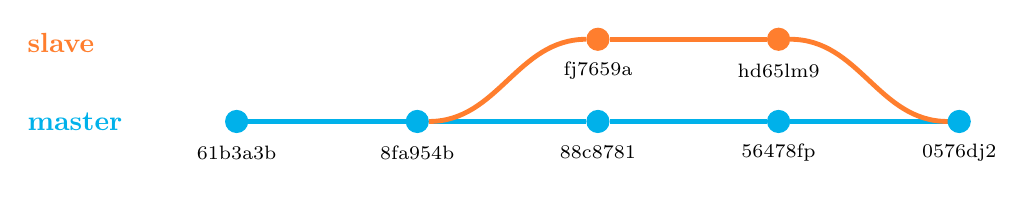
\begin{tikzpicture}

	%%% master branch
	% nodes and hashes
	\node[cmaster] 				(m0) at (0,0) 	{};
	\node[hash] (m0t) at (m0.south) {61b3a3b};
	
	\node[cmaster, right=of m0] 	(m1) 			{};
	\node[hash] (m1t) at (m1.south) {8fa954b};

	\node[cmaster, right=of m1] 	(m2) 			{};
	\node[hash] (m2t) at (m2.south) {88c8781};
	
	\node[cmaster, right=of m2] 	(m3) 			{};
	\node[hash] (m3t) at (m3.south) {56478fp};
	
	\node[cmaster, right=of m3] 	(m4) 			{};
	\node[hash] (m4t) at (m4.south) {0576dj2};
	
	% branch
	\draw[bmaster] (m0) to[out=0,in=180] (m1);
	\draw[bmaster] (m1) to[out=0,in=180] (m2);
	\draw[bmaster] (m2) to[out=0,in=180] (m3);
	\draw[bmaster] (m3) to[out=0,in=180] (m4);
	
	% name
	\node[nmaster, left=of m0] (mn) {master};
	
	%%% top daughter branch
	% nodes and hashes
	\node[ctop, above=of m2]		(t2) 		 	{};
	\node[hash] (t2t) at (t2.south) {fj7659a};
	
	\node[ctop, above=of m3]		(t3) 		 	{};
	\node[hash] (t3t) at (t3.south) {hd65lm9};
	
	%. branch
	\draw[btop] (m1) to[out=0,in=180] (t2);
	\draw[btop] (t2) to[out=0,in=180] (t3);
	\draw[btop] (t3) to[out=0,in=180] (m4);
	
	% name
	\node[ntop, above=of mn] (tn) {slave};
    
\end{tikzpicture}
%%%%%%%%%%%%%%

\end{document}